% Chapter III:
\section{Marco Teórico}

\subsection{Antecendentes del Problema}

\lipsum[15]

\lipsum[15]

\subsection{Bases Teóricas}

\lipsum[2]

\subsection{Marco Conceptual}

Table~\ref{tab:BasicTable} summarizes the data. \lipsum[15]

\begin{table}
  \caption{Sample Basic Table}
  \label{tab:BasicTable}
  \begin{tabular}{@{}llr@{}}         \toprule
  \multicolumn{2}{c}{Item}        \\ \cmidrule(r){1-2}
  Animal    & Description & Price \\ \midrule
  Gnat      & per gram    & 13.65 \\
            & each        &  0.01 \\
  Gnu       & stuffed     & 92.50 \\
  Emu       & stuffed     & 33.33 \\
  Armadillo & frozen      &  8.99 \\ \bottomrule
  \end{tabular}
\end{table}

\begin{figure}[!ht]
	\centering
  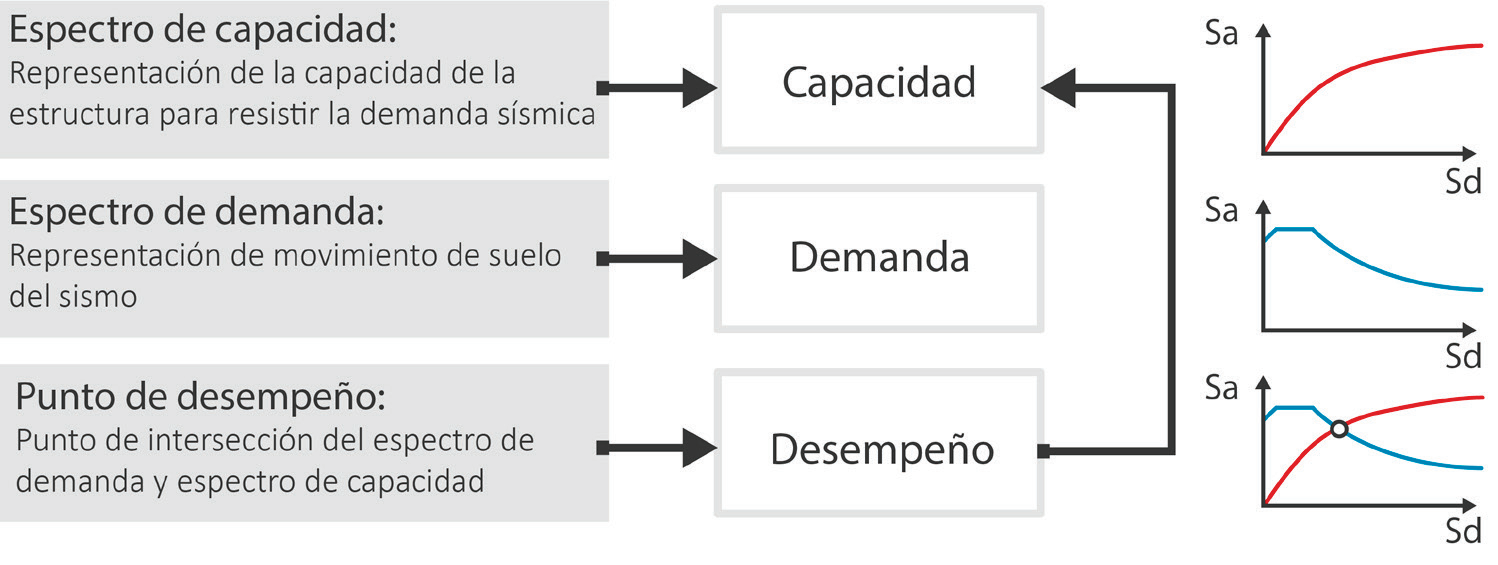
\includegraphics[scale=0.36]{E_IMAGENES/3_Capitulo3/Cap3_Imagen70.png}
	\caption{\centering\footnotesize Cuadro y gráficos que. Adaptado de \cite{deWaal2009}}
  \figurenote{This is a great figure.}
	\label{Cap3_Figura2}
\end{figure}

Figure~\ref{Cap3_Figura8} shows this trend. \lipsum[16]